\chapter*{General Introduction}
\addcontentsline{toc}{chapter}{General introduction}

Reading is a complex and unique skill of the human brain. Reading aloud requires the brain to perform multiple low and high level processes, such as graphical pattern recognition, composition of letters into words, grapheme-to-phoneme conversion, phoneme production and, regularly, ascription of meaning – all almost in parallel and in strikingly short time and accuracy. Reading is thus a fertile ground for studying many processes that take place in the brain. Much can be learned about our visual, auditory, and motor systems, and their interactions, from the understanding of reading processes.

Research on reading focuses on both normal and abnormal reading. The study of abnormal reading, such as in the case of dyslexia, has been highly contributional to theoretical understanding of the process of reading itself, as well as for clinical purposes. Insights about the processes underlying normal reading were often derived from the analysis of data such as reading errors \citep{mn73, ck12}, reaction times \citep{s98, s00} and eye movements \citep{jainta2011dyslexic}, during reading of dyslexic people. Similarly, in neuroscience, studies of reading have explored brain activity of both normal and dyslexic subjects \citep{gaab2007neural, shaywitz2002disruption, price2012review}.

To this day, research on reading and dyslexia has reached major insights, suggesting general cognitive theories \cite{stanovich1988explaining, vellutino1995semantic, ramus2003relationship, amitay2003reply, ck12}, characterization of the neuronal activity involved in the process \citep{joubert2004neural, gaab2007neural, dehaene2010children}, and possible clinical interventions \citep{coltheart1989treatment, aylward2003instructional, kipp2008remediation}. However, to this day, there is no consensus on one theory of reading and dyslexia. In fact, the term 'dyslexia' has received a multitude of definitions and descriptions in the literature, and various theories have been proposed to account for related behavioral findings, and have suggested various underlying causes of dyslexia \citep{eg14}. This fact also impacts the interpretation of results from neuroscience, as the definition of the deficit of subjects participating in the experiments depends on the theoretical school you ask. 

Accepted theories of dyslexia today span from single-cause \citep{stanovich1988explaining, s98, s00} and dual-cause \citep{wolf1999double}, to multifactorial-cause theories \citep{ck12}. The single-cause theory proposes that dyslexia is caused by a general phonological deficit and may be assessed by measuring reading accuracy and reaction time. The multifactorial-cause theory proposes to discern the term dyslexia into various subtypes with different causes, each characterized by making a specific type of errors. As opposed to single-cause theories, the subtype approach to dyslexia analyzes the types of errors made by dyslexia people. For example, the word {\it leaf} can be read as 'lead', as 'leave', or as 'loaf', and the word {\it bear} can be read as 'bean', as 'pear', or as 'bare'. The first type of error in both cases can be characterized as consonant letter substitution, the second as voicing substitution (since both phoneme pairs /f/-/v/ and /b/-/p/ differ by the voicing feature), and the third as vowel substitution. According to this theory, specific types of errors point to specific sub-processes in normal reading, which are selectively impaired in different subtypes of dyslexia. In sum, whether dyslexia has a single cause or should be discerned into subtypes remains a controversial issue in the field.

Joining this wider theoretical question, other more specific questions remain in the field. In particular, with regards to the subtype approach to dyslexia, questions remain regarding specific subtypes of dyslexia, as described in the following, after a short background on the subtype approach: The first researchers to distinguish different subtypes of dyslexia, and the first to propose a cognitive model of reading, which accounts for these different subtypes were \citet{mn73}. The model proposed was a Dual-Route model, in which reading takes place in two routes, activated in parallel upon reading. One route, the lexical route, serves for reading already known words, and is characterized by fast retrieval of words from long-term memory lexicons. The second route, the sub-lexical route, serves for reading new, non-familiar words, and is characterized by step-by-step conversion of graphemes to phonemes. In this model, each subtype of dyslexia, associated with specific error types, was to be explained by a malfunction of a specific locus in the model. With time, the discovery of new characteristic error types, that is, new subtypes of dyslexia, led to the modification and refining of the reading model. Figure 1 describes the most accepted version of the Dual-Route Model. 

\begin{figure}[h]
\vspace{.3in}
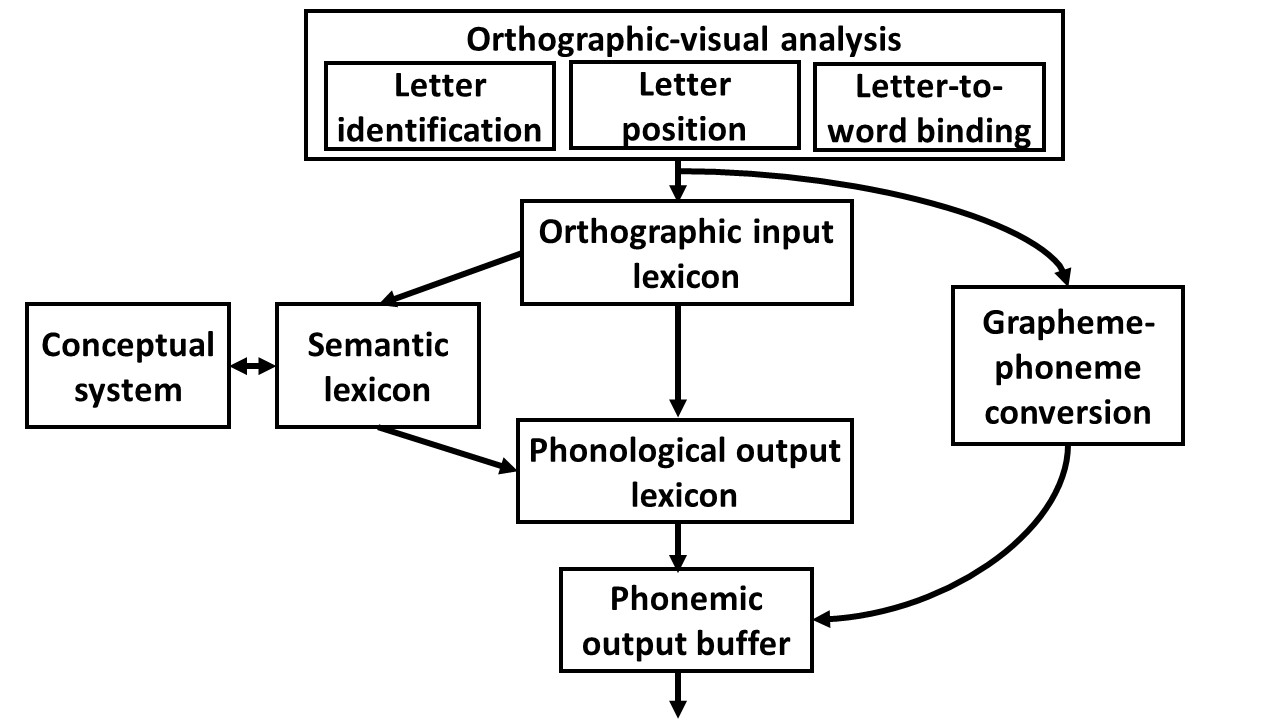
\includegraphics[width=\linewidth]{Figures/Ch1/DualRoute}
\caption{The dual-route model \citep{friedmann2016types}}
\end{figure}

With regards to the sub-lexical route, a general malfunction identified several decades ago, is called Phonological Dyslexia (for review, see \citealp{c96}). Individuals with this type of dyslexia can read words with which they are already familiar (words that exist in their orthographic input and phonological output lexicons – Figure 1), but they make errors in reading non-familiar words. The hypothesized cause for these errors is a general malfunction related to the conversion of graphemes into phonemes. Recently, more specific subtypes of dyslexia of the sub-lexical route were reported, all characterized by malfunctions related to specific phonological features: \citet{Gvion2010} reported a person with selective conversion impairment reading ‘goat’ as ‘coat’ and ‘pear’ as ‘bear’ thus having voicing substitution errors. They therefore coined this subtype of dyslexia as ‘Dyslegzia’. \citet{Gvion2012} reported  a case in which only the nasality feature was affected (alongside the voicing feature), naming this dyslexia as 'Nasalexia'. Last, \citet{kf11} reported a new sub-lexical route dyslexia, in which only vowels are affected and not consonants, called, Vowel Letter Dyslexia. They reported 25 cases of individuals making errors of migrations, substitutions, omissions, or additions of a vowel letter, and showed, as for all the above subtypes of dyslexia, converging evidence that the impairment was located in the sub-lexical route and not in a different locus of the Dual-Route reading model. These subtypes of dyslexia - dyslegzia, nasalexia, and vowel-letter dyslexia - show impairments with respect to specific phonological features - voicing, nasality and vowels, correspondingly (recent evidences of substitutions among strident phonemes were also observed \citealp{Gvion2010}). All errors in these phonological feature-based dyslexia subtypes are characterized by mapping a letter to an erroneous phoneme that differs from the correct one by a single phonological feature, as in dyslegzia and nasalexia, or to an erroneous phoneme that belongs to the same natural class of the correct one, as in the case of vowels and stridents. Importantly, there are currently no known subtypes of dyslexia that specifically affect other phonological features. For example, there is no evidence for a deficit that generates phoneme substitutions related to the [labial] feature. It is currently unclear as to why some feature-based errors are more common in reading than others, and what is the underlying phonological structure that causes this discrimination. These sorts of questions and their research may now have an important contribution to the detailed understanding of reading, as the current scientific goal is to characterize the exact building blocks of these intricate processes.

The answer to the question regarding feature-based subtypes of dyslexia may lie in the similarity relations among phonemes. The related reading errors may follow phoneme similarity, since phonemes that are more similar to each other may be more prone to participate in substitution errors. Various studies have suggested means to measure phoneme similarity in an experiment \citep{NicelyMiller1955, Luce1987, cutler2004patterns} by presenting noise-corrupted versions of phonemic stimuli to normal subjects, then inferring about phoneme similarity from confusion rates among stimuli \citep{Tversky1977}. However, given such estimations of phoneme similarity, it stays unclear what is the contribution of each feature to the overall similarity. A difference with respect to some phonological features may make a pair of phonemes more perceptually distinguishable, or similar, compared to pairs that differ in other features. For example, a difference with respect to nasality ([+nasal] vs. [-nasal]) as in /n/-/d/, may render the two more distinguishable compared to a difference with respect to, e.g., [labial] as in /n/-/m/. Since such differences may explain prevalence of feature-based subtypes of dyslexia, it seems crucial to quantify the contribution of various phonological features to the overall similarity.

In sum, in the center of this thesis and motivating the questions it addresses is the rich phenomenology of error types in dyslexia. The question of the heterogeneity of dyslexia, and that of the existence of specific feature-based subtypes, are hereby addressed. In common to both investigations, the thesis adopts a novel methodological approach to reading, which designs data-driven computational models to study these questions. The field of data-driven models has gone through a recent rapid growth and development in various scientific fields, but was hardly adopted to explore questions regarding reading and its disorders. As described below, this methodology may provide new insights about persisting questions and debates in the field.

With the advancement in computing technologies, computational models of cognitive functions have widely spread in research, and so have computational models of reading become an acknowledged approach for investigating  reading and its disorders. Computational models enjoy several advantages over traditional theories, which complement box-and-arrows models as that of the Dual-Route model. First, they propose detailed simulations of normal human performance and allow the introduction of lesions into the simulations, which can then be compared to behavioral data collected from neuropsychological patients. Second, computational models are considered to be highly explicit, as they need to be specific about various implementational details, such as characteristic processing times and dynamics of their units. Finally, they propose falsifiable predictions, which are quantitative compared to those of verbal theories. These have made computational models highly influential on the field.

In the field of computational modelling, a family of computational models which possesses its own unique advantages, is that of data-driven models. Data-driven models are based on learning algorithms, and are typically trained on large corpora of data from which they can extract various types of information. They usually require a relatively small number of prior assumptions about the process in question, and are therefore occasionally described under the slogan of: 'letting the data speak for itself'. As a scientific approach, the data-driven approach is contrasted to the traditional hypothesis-driven one, and was suggested by some researches as an essential component in scientific research \citep{kell2004here}. Data-driven models have had tremendous success and have rapidly spread in other fields \citep{bell2009beyond, leonelli2014difference, lecun2015deep}. However, to this day, they have received minimal attention in the field of reading disorders. With the accumulation of data on reading, it seems that applying a data-driven approach to yet existing research questions in the field, may reach novel insights and may open new research paths.

This thesis addresses open questions in the field of reading disorders through the construction of data-driven computational models. To address the question regarding the heterogeneity of dyslexia, chapter 1 presents data-driven models to the problem, which are trained on a large corpus of reading-error data. By this, it proposes a new approach to the persisting debate by letting the data "to speak for itself". More specifically, this chapter explores the generation process of reading-errors with probabilistic graphical models, making use of probability language to capture the complex generation process of reading errors. The learning algorithms used to train the models can discover possible hidden patterns in the data, thus shedding light on the issue in question. In addition, the study develops an automatic diagnostic tool of subtypes of dyslexia, based on error types, which lays the groundwork for easily accessible, cheap and fast screening tests. 

To address the question regarding the existence of specific feature-based subtypes of dyslexia, the next two chapters characterize phoneme similarity based on behavioral and neural data: the behavioral data is composed of a phoneme-confusion dataset that we have collected for Hebrew, and of existing similar datasets in English, on which we test our approach. The neural data is composed of electrophysiological recordings of spiking neuronal activity in high-level auditory regions of the superior temporal gyrus (STG) of humans, which presumably reflects phoneme perception. 

chapters 2 presents data-driven models to the problem of phoneme similarity. It therefore differs from previous studies in phonology, which manually designed similarity functions (e.g., \citealp{Pierrehumbert1993, Frisch1997}). In this chapter, we explore several methods to learn a metric defined over pairs of phonemes from phoneme-confusion data. Comparing the results, we identify the most suitable method for further analyses, and describe the contribution of each phonological feature to the overall similarity. Next, to see whether the contribution of a phonological feature may differ across languages, we compare results from English and Hebrew. 

Chapter 3 complements the inquiry into phoneme similarity from a neuroscientific point of view, by analyzing spiking activity recorded in the human STG during a listening task, using depth electrodes. Such invasive electrophysiological recording techniques provide a rare glimpse into neural processes underlying the unique language capacity of humans, and in particular, a precious opportunity to study phoneme representations in the human brain. Recent studies, using electrocorticography (ECoG) subdural grids, have provided a detailed description of phoneme representations in the STG during listening to natural speech \citep{pasley2012reconstructing, Mesgarani2014}. Interestingly, results of these studies also suggest that phoneme representations are acoustic based, as auditory theories to speech perception suggest \citep{stevens1972quantal, stevens1989quantal}, and are in contrast with speech-perception theories suggesting that during listening the hearer extracts intended motor gestures of the speaker \citep{liberman1967perception, liberman1985motor}. Specifically, \citet{Mesgarani2014} shows that manner-of-articulation features, which have clear acoustic correlates, dominate the functional organization of phonemes in the STG. Remarkable as these results are, electrical activity recorded in ECoG grids only reflects average responses of large neuronal populations, and is commonly analyzed into the gamma band only. It therefore remains unclear how single cells in the STG represent phonemic stimuli, and what are the phonological features that dominant these representations. Describing and construing single-cells activity is indispensable for a complete theory of the neural basis of speech perception, and cognitive processes in general. 

\citet{fried1999cerebral} have developed a novel technique, using depth electrodes, to obtain multiple single-unit recordings from the cortex and deep brain structures in humans. This technique provides unique spatiotemporal resolution to probe into neural activity, in this case, neural activity underlying phoneme processing. Chapter 3 tests the dominance of various phonological features in neural representations of phonemes, by analyzing spiking activity recorded while aurally presenting consonant-vowel and vowel stimuli to neurosurgical patients implemented with depth electrodes. In this chapter, we characterize the functional organization of phonemes from spiking activity, and quantify the dominance of various phonological features in the neural representations. Next, we compare the neural representations and the perceptual similarities among phonemes from chapter 2. Taken together, these two chapters provide a characterization of both neural and cognitive similarity structures among phonemes. 

Finally, having a rare glimpse into single-cell responses in the human STG to phoneme stimuli, we also draw on the results to address the long lasting debate in the field of speech perception, whether phoneme perception is based on identifying underlying motor gestures \citep{liberman1967perception, liberman1985motor} or acoustic cues \citep{stevens1972quantal, stevens1989quantal}, as described above. To this end, we test whether the dominating phonological features that we find in neural data are in accordance with motor theories, or rather, with auditory theories to speech perception. If neural activity in high-level auditory regions of the STG reflects phoneme perception, motor theories would predict a functional organization of phonemes in the STG that is based on place-of-articulation features, such as [labial] or [palatal], whereas auditory theories would predict a functional organization that is based on manner-of-articulation features such as [nasal] and [plosive]. We test both predictions by exploring the functional organization of phonemes revealed by the data of single-cell recordings.